\documentclass[11pt]{article}
\usepackage[utf8]{inputenc}
\usepackage[margin=2.5cm]{geometry}
\usepackage{amsmath,amsthm,amsfonts,amssymb}
\usepackage{graphicx,latexsym}
\usepackage{float}
\usepackage{booktabs}
\usepackage{multirow}
\usepackage{cite}
\usepackage{url}
\usepackage{algorithm}
\usepackage{algpseudocode}
\usepackage{caption}
\usepackage{tikz}
\usetikzlibrary{arrows.meta,positioning,fit,backgrounds}
\renewcommand{\baselinestretch}{1.2 }

% ---------------------------------------------------------------------------
% REFRAME v2 (journal-agnostic). Changes vs main_v1_backup.tex:
%   - Abstract reframed: architectural pattern + gap-to-failure diagnostic as
%     the headline; F1 numbers demoted to a supporting pilot result.
%   - Contributions rescoped to what the evidence supports.
%   - Evaluation restructured for multi-topic + a matched scored-grounding
%     ablation. Single-topic numbers retained as "Topic 1 (pilot)".
%     Sections marked % [PENDING] are filled from eval/results/matrix_*/aggregate.md
%     once eval/run_matrix.py has been run (see eval/README.md).
%   - Limitations -> "Threats to Validity"; fixed defects moved to a footnote.
%   - Added Reproducibility subsection.
% Bump \NumTopics and \NumRuns when the matrix run lands.
% ---------------------------------------------------------------------------
\newcommand{\NumTopics}{one}     % -> "five" after multi-topic run
\newcommand{\NumRuns}{three}     % -> "five" after run_matrix --repeats 5

\title{\textbf{Reject-Before-Propagate: Build-Time Citation Gates for
Agentic Literature-Synthesis Pipelines}}

\author{\begin{tabular}{rcl}
\textbf{Harish Vidyarth N$^{\text a,}$\thanks{Corresponding author: harishvidyarth.n.2024.csecs@rajalakshmi.edu.in}, A.L. Reshma$^{\text a}$, R. Divya$^{\text a}$}
\end{tabular}\\
\\
\begin{tabular}{c}
$^{\text a}$\small Department of Computer Science and Engineering (Cyber Security), \\Rajalakshmi Engineering College, Thandalam, Chennai 602105, India \\
\end{tabular}}

\date{}

\begin{document}
\maketitle
\vspace{-0.5cm}
\begin{abstract}
{\small Large language model (LLM) pipelines for automated literature review
increasingly chain several generative stages -- claim extraction, contradiction
detection, evidence synthesis -- whose outputs are consumed by downstream stages
and, ultimately, by people making real decisions. In current systems, citation
grounding is treated as a \emph{scored} property: a generated statement is
checked against retrieved evidence and assigned a confidence value, flagged, or
routed for human review, but is not structurally prevented from reaching the
final output when that check fails. We describe \textbf{Verify-or-Reject
Grounding (VoRG)}, an architectural pattern that instead treats citation
grounding as a \emph{build-time invariant}: each pipeline stage either produces
output whose type excludes unverifiable content -- because the stage is
deterministic over already-verified inputs, or because an explicit check
discards non-conforming output before it can propagate -- or it raises a build
error. We give a formal statement of the pattern, a linear-time certification
algorithm for its narrative-verification instance, and a reference
implementation that applies it to three subsystems of an eight-stage
research-assistant pipeline (evidence-grounded synthesis, contradiction
detection, and journal-metadata reconciliation). We evaluate on \NumTopics{}
gold-annotated topic(s) with \NumRuns{} repeated runs per configuration,
comparing the gated pipeline against a matched \emph{scored-grounding} ablation
that keeps the same stage decomposition but replaces each rejection with a
confidence score, and against a naive single-prompt baseline. The most robust
finding is diagnostic rather than a headline metric: the pipeline stages
protected by a verify-or-reject gate produce no output contradicted by the
reviewed corpus, while research-gap detection -- the one major stage with no
such gate -- produces a confirmed false claim directly contradicted by a paper
already in the corpus. This gap-to-failure correspondence, between which stages
are architecturally protected and where empirical failures occur, is reported as
a concrete design finding and motivates extending the same discipline to every
generative stage of an agentic scientific-NLP pipeline.}
\end{abstract}
\textbf{Keywords:} {\small verify-or-reject grounding; literature synthesis; large language models; citation grounding; hallucination mitigation; agentic NLP; scientific NLP}

\section{Introduction}

Large language models are increasingly used to accelerate literature review by
extracting claims from papers, identifying disagreements between studies, and
drafting synthesis narratives. A well-documented failure mode of this automation
is \emph{hallucination}, in which a generated statement appears well supported
but does not correspond to any statement in the
source~\cite{zhang2025hallucination,ji2023survey,tonmoy2024comprehensive}. A
closely related failure is citation-level: even when the surrounding text is
accurate, the cited source may not actually say what the model claims, or may
not exist at all~\cite{zhang2025citation}. Existing mitigation approaches
commonly rely on post-hoc verification, in which a claim or generated passage is
checked against retrieved evidence and assigned a score, flagged, or routed for
human review~\cite{li2025enhancing}. Because validation in this scheme is a
signal appended to the output rather than a gatekeeper that controls it, an
unverified or contradictory statement can still reach the user if the score is
not acted on.

This paper describes an alternative design principle, \textbf{Verify-or-Reject
Grounding (VoRG)}. The distinction matters because synthesis output from
pipelines of this kind is often consumed downstream by people making real
decisions, such as a systematic-review team drafting a
submission~\cite{li2025enhancing}; a hallucinated citation that merely lowers a
confidence score, rather than being blocked outright, carries a correspondingly
higher cost in that setting. Section~\ref{sec:method} formalizes VoRG's
rejection semantics and gives a linear-time certification algorithm for the
narrative-verification case. Section~\ref{sec:evaluation} reports a reproducible
evaluation whose most informative result is a correspondence between
architectural coverage and failure location rather than an effect size.

Our contributions are:
\begin{enumerate}
 \item A formal statement of Verify-or-Reject Grounding as a reusable
 architectural pattern (\S\ref{sec:method}), distinguished from scored or soft
 grounding by its build-time rejection semantics, together with
 \textsc{VoRG-Certify}, an $O(n+M)$ narrative-certification algorithm that
 removes the $O(n\cdot m)$ term implicit in a naive per-sentence evidence scan.

 \item A reference implementation applying the pattern to three subsystems of an
 eight-stage research-assistant pipeline -- evidence-grounded synthesis,
 contradiction detection, and journal-metadata reconciliation
 (\S\ref{sec:architecture}) -- released with its evaluation harness and
 gold-annotation files.

 \item A reproducible evaluation (\S\ref{sec:evaluation}) that compares the
 gated pipeline against a \emph{matched scored-grounding ablation} -- the same
 stage decomposition with every rejection replaced by a confidence score -- and
 a naive single-prompt baseline, and reports a \textbf{gap-to-failure
 correspondence}: the verify-or-reject-gated stages produce no output
 contradicted by the reviewed corpus, whereas the single ungated stage produces
 a false claim that a corpus paper directly contradicts.
\end{enumerate}

The remainder of the paper is organized as follows.
Section~\ref{sec:related} reviews related work on automated literature review,
contradiction detection, citation grounding, and bibliometric reconciliation.
Section~\ref{sec:architecture} describes the system architecture,
Section~\ref{sec:method} presents the verify-or-reject pattern and its
certification algorithm, and Section~\ref{sec:evaluation} reports the
evaluation. Discussion, threats to validity, and reproducibility are presented
in Sections~\ref{sec:discussion}--\ref{sec:repro}, followed by the conclusion.

\section{Related Work}
\label{sec:related}

\textbf{AI-assisted systematic review.} Li et al.~\cite{li2025enhancing} develop a GPT-4-driven, five-module system (literature search, PICOs criteria setup, abstract screening, data extraction, and reporting) for systematic literature reviews conducted as part of health technology assessment (HTA) submissions, with a human-in-the-loop design that permits real-time criteria refinement. Evaluated on 3{,}713 relapsed/refractory multiple myeloma abstracts and 1{,}720 advanced-melanoma abstracts, the system reports 90\% average sensitivity (82 to 97\%) and an F1 score of 82 (69 to 90) for abstract screening, and an F1 score of 93 (precision 91\%, recall 94\%) for data extraction. These figures show the system performs well within its evaluated domain, but its grounding safeguard is a human review step, not a structural constraint on what the model can emit: a low-confidence screening or extraction decision is still surfaced to the reviewer rather than withheld. This is the closest published system to the reference implementation described here and is treated as this paper's base comparison: where Li et al.~\cite{li2025enhancing} score output and route it for human review, our pipeline rejects unverifiable output automatically, without a human in the loop at generation time. Two more recent LLM-assisted review tools broaden this landscape without changing the underlying pattern: Haryanto's LLAssist~\cite{haryanto2024llassist} automates relevance screening and information extraction with an LLM scoring each paper's fit to a research question, and Scherbakov et al.~\cite{scherbakov2025emergence} systematically review 172 LLM-automated-review studies and find that the large majority automate a single stage (most often search or data extraction) with a confidence score or human check, rather than a chained, structurally-gated pipeline.

\textbf{Automation of systematic review more broadly.} van Dinter et al.~\cite{vandinter2021automation} systematically review the SLR-automation literature and find that most automation efforts target individual review stages (search, screening, or data extraction) in isolation, with few systems chaining verifiable stages end-to-end into a single pipeline with consistent grounding guarantees, a gap the architecture in \S\ref{sec:architecture} is designed to close. The broader retrieval-augmented and agentic-LLM literature offers relevant building blocks without addressing this gap directly: retrieval-augmented generation~\cite{lewis2020retrieval} grounds generation in retrieved passages but does not reject ungrounded output, ReAct-style tool-using agents~\cite{yao2023react} interleave reasoning and external actions without a citation-level accept/reject rule, and Self-RAG~\cite{asai2024selfrag} trains a model to critique its own retrieval and generation via learned reflection tokens, which is closer in spirit to VoRG but remains a soft, learned signal rather than a hard, external verification gate.

\textbf{Contradiction detection.} Alamri and Stevenson~\cite{alamri2016contradiction} survey technologies for detecting contradictory claims in biomedical literature, cataloguing linguistic and statistical approaches that predate LLM-based judgment and that do not incorporate an explicit reject path for low-confidence judgments: a contradiction is asserted or not, with no abstention option grounded in evidence availability. The natural-language-inference literature underlying most modern contradiction detectors, exemplified by the MultiNLI corpus~\cite{williams2018broad}, treats contradiction as a three-way classification (entailment, neutral, contradiction) rather than as a judgment that can itself be withheld when supporting evidence is thin, and using an LLM as the judge introduces its own reliability question~\cite{zheng2023judging} that a bare classification score does not surface. We were unable to locate a Q1-indexed journal paper specifically addressing LLM-based contradiction judgment with an explicit grounding/rejection mechanism; this appears to be an open area, which we report as such rather than citing an unpublished preprint to fill the gap.

\textbf{Citation faithfulness and reporting transparency.} The PRISMA-trAIce checklist~\cite{prismatraice2025} proposes standardized disclosure of how AI was used at each stage of a systematic review. This is complementary to, but distinct from, our concern: PRISMA-trAIce standardizes what authors \emph{report} about AI use, whereas VoRG constrains what the \emph{system itself} is structurally permitted to output. Zhang and Zhang~\cite{zhang2025hallucination} review RAG hallucination-mitigation techniques generally, a landscape further mapped by Ji et al.'s taxonomy of hallucination types~\cite{ji2023survey} and Tonmoy et al.'s survey of over thirty mitigation techniques~\cite{tonmoy2024comprehensive}; benchmarks such as TruthfulQA~\cite{lin2022truthfulqa} and HaluEval~\cite{li2023halueval} quantify how often models produce unsupported content, and SelfCheckGPT~\cite{manakul2023selfcheckgpt} detects it post hoc by sampling multiple generations and checking their consistency -- all of these score or detect hallucination rather than structurally blocking it. Closer to citation grounding specifically, Rashkin et al.'s Attributable-to-Identified-Sources framework~\cite{rashkin2023measuring} and Bohnet et al.'s Attributed Question Answering task~\cite{bohnet2022attributed} formalize how to \emph{measure} whether a generated statement is attributable to a source, Gao et al.'s ALCE benchmark~\cite{gao2023enabling} finds that even strong LLMs leave citation claims unsupported roughly half the time on open-ended questions, Press et al.'s CiteME benchmark~\cite{press2024citeme} shows frontier models correctly identify a cited paper only 4--19\% of the time versus 70\% for humans, and Zhang and Zhao~\cite{zhang2025citation} document well-formatted but fabricated references as a recurring LLM failure mode in academic writing. VoRG differs from all of the above in the same way: these are measurement and detection tools, reporting how faithful or attributable an output is, whereas VoRG is a build-time gate that prevents an unattributable statement from being emitted at all.

\textbf{Journal-metadata reconciliation.} Mach\'a\v{c}ek and Srholec~\cite{machacek2022predatory} document substantial cross-country and cross-database inconsistency in how predatory or borderline journals are classified in Scopus, and Mongeon and Paul-Hus~\cite{mongeon2016journal} independently find that Web of Science and Scopus disagree sharply in which journals they index at all, with English-language and STEM journals systematically overrepresented in both -- together motivating systems that reconcile multiple bibliometric sources explicitly rather than trusting a single database. Chen et al.~\cite{chen2023open} build an automated predatory-journal classifier from blacklist/whitelist text features, which is a useful point of contrast: their system outputs a binary predatory/not-predatory prediction, whereas the journal-metadata subsystem described in \S\ref{sec:architecture} applies the verify-or-reject discipline to a different question -- a metric is reported only when a source explicitly provides it, and conflicting sources are surfaced in a discrepancy field rather than silently averaged or classified away. The Scientometrics editorial~\cite{scientometrics2025editorial} frames AI-assisted bibliometrics as an emerging area generally, without a specific method for gap detection; we found no dedicated Q1-journal paper on automated research-gap mining from literature corpora, which we note as a genuine open area rather than force an imprecise citation.

Existing research has thus addressed several parts of automated literature review, including literature screening, information extraction, contradiction detection, hallucination mitigation, and bibliometric analysis, and has improved the efficiency of individual stages. Verification in these systems, however, is generally treated as a score, a review step, or a separate validation process rather than as a requirement that controls whether an output can proceed to the next stage; as a result, an unsupported statement may still pass through the pipeline if the verification step only reports its confidence or flags it for later review. This leaves a gap in enforcing citation grounding as a structural property across an automated research pipeline; Sections~\ref{sec:architecture} and~\ref{sec:method} describe how the present work closes it.

\section{System Architecture}
\label{sec:architecture}

The reference system is a research-assistant pipeline with eight sequential stages: topic expansion, multi-source paper discovery, claim extraction, claim normalisation, contradiction detection, research-gap detection, citation building, and persistence. Framing pipeline quality as reproducible, stage-level evaluation rather than an end-to-end demo follows the practice recommended by agentic-LLM evaluation frameworks such as AgentBench~\cite{liu2024agentbench}, which likewise scores an LLM system stage by stage against fixed environments rather than by inspecting final output alone. Within this pipeline, three subsystems implement the verify-or-reject pattern explicitly: evidence-grounded synthesis, contradiction detection, and journal-metadata reconciliation; the remaining five stages, described below, are ordinary generation or aggregation steps that feed into those gates.

\textbf{Topic expansion.} An LLM decomposes the input topic into a structured map of 3--6 subtopics, 2--6 methods, up to 6 benchmark datasets, and 6--12 search keywords, with an explicit prompt instruction not to invent a dataset name it is not confident exists -- a prompt-level echo of the grounding discipline enforced structurally elsewhere in the pipeline, though not itself a hard gate. When no LLM provider is configured, or the call fails to parse, the system falls back to a hardcoded five-domain keyword dictionary; this fallback is independently selectable via an environment flag and is also the rule-based configuration used for the pattern-mode ablation in \S\ref{sec:evaluation}.

\textbf{Multi-source paper discovery.} The live system queries arXiv, Semantic Scholar, and CrossRef concurrently, merging results into one common schema and deduplicating by DOI match, normalized title match, and fuzzy title similarity within a one-year publication-date window; a fourth source, PubMed, is implemented but currently disabled because its detail-retrieval step returns placeholder titles that would poison downstream claim extraction, and three further sources (Springer, Elsevier, Wiley) are scaffolded pending API keys. Each frozen gold corpus used in \S\ref{sec:evaluation} is retrieved once and cached; when a record lacks an abstract after the CrossRef merge, the snapshot tool backfills abstract text from the Semantic Scholar and OpenAlex APIs before freezing, and the resulting abstract coverage is recorded with the snapshot.

\textbf{Claim normalisation.} Before claims reach contradiction detection, a normalisation stage folds metric-name synonyms (e.g. ``acc'', ``f-score'' $\to$ a single canonical name per metric) and units (percentages to decimals) into a common vocabulary, and computes a rule-based confidence adjustment from the claim's own wording: hedging language (``might'', ``possibly'') lowers confidence, strength language (``demonstrates'', ``outperforms'') and statistical-significance markers (``p $<$'', ``confidence interval'') raise it. This is deliberately a \emph{scored}, not gated, step -- it adjusts a confidence value rather than rejecting a claim -- and sits directly upstream of the gated contradiction-detection stage, illustrating the contrast formalized in \S\ref{sec:method}.

\textbf{Citation building.} A dedicated agent renders each discovered paper's metadata into BibTeX, APA, IEEE, and MLA formats, selecting a venue-aware template (journal, conference, or arXiv preprint) per paper; a separate formatter handles author-name and DOI-link normalization for the export path. This stage is a deterministic transformation of already-verified paper metadata, not a new hallucination surface.

\textbf{Persistence.} Two storage layers back the pipeline. Run-level state (topic map, discovered papers, claims, contradictions, research gaps) is written to JSON files rather than a binary format, a deliberate choice for stability across Python versions. Journal-quality data is instead kept in a relational schema with one table per external source (SCImago, Scopus Master Journal List, DOAJ, Anna University's approved-journal list, and per-publisher article-processing-charge lists), joined on ISSN to a canonical journal record; every source row carries its own snapshot date and source URL, and a consolidated view records an explicit confidence tier (verified, estimated, or unknown) plus a free-text discrepancy note rather than silently overwriting a conflicting figure. This extends the same never-merge-silently discipline described below for journal-metadata reconciliation down into how the data is actually stored, not just how it is queried.

The evidence-grounded synthesis sub-pipeline, the most detailed of the three VoRG-gated subsystems, is shown in Figure~\ref{fig:architecture}.

\textbf{Evidence-grounded synthesis sub-pipeline.} An evidence-extraction stage pulls structured claims (population, method, dataset, metric, result, limitation) from each paper, and every extracted field is checked as a verbatim or near-verbatim substring of the source text before being admitted to an evidence table; nothing enters the table on the strength of paraphrase alone, a check structurally analogous to the evidence-retrieval step in fact-verification tasks such as FEVER~\cite{thorne2018fever}, except that here an unsupported extraction is discarded rather than scored as ``not enough info''. A synthesis-matrix stage then aggregates evidence rows into a methods-by-datasets grid, classifying each cell as agreement, conflict, or blank; this stage is deterministic (no LLM call), which removes an entire class of hallucination risk from what is otherwise the most aggregation-heavy step of the pipeline. Finally, a narrative-generation stage drafts prose citing evidence rows, and a narrative-verifier stage mechanically rejects any generated sentence whose citation key does not resolve to a row in the verified evidence table; an unsupported sentence is treated as a build error, not a warning.

\textbf{Contradiction detection.} Candidate claim pairs are pre-filtered by TF-IDF similarity to bound the search space, then judged by an LLM on an 11-point Likert contradiction scale with an explicit contradiction-type classification (direct, conditional, or methodological). Judgments below a likelihood threshold are discarded rather than reported with low confidence.

\textbf{Journal-metadata reconciliation.} A separate subsystem merges journal-quality signals (SCImago, Scopus Master Journal List, DOAJ, per-publisher article-processing-charge data, and an OpenAlex-derived citation-rate estimate) using a precedence rule, and flags cross-source discrepancies above 10\% rather than resolving them silently. Metrics are reported in one of three explicit confidence tiers: verified, estimated, or unknown, so a missing or unverifiable figure surfaces as ``unknown'' rather than being interpolated.

\begin{figure}[ht]
\centering
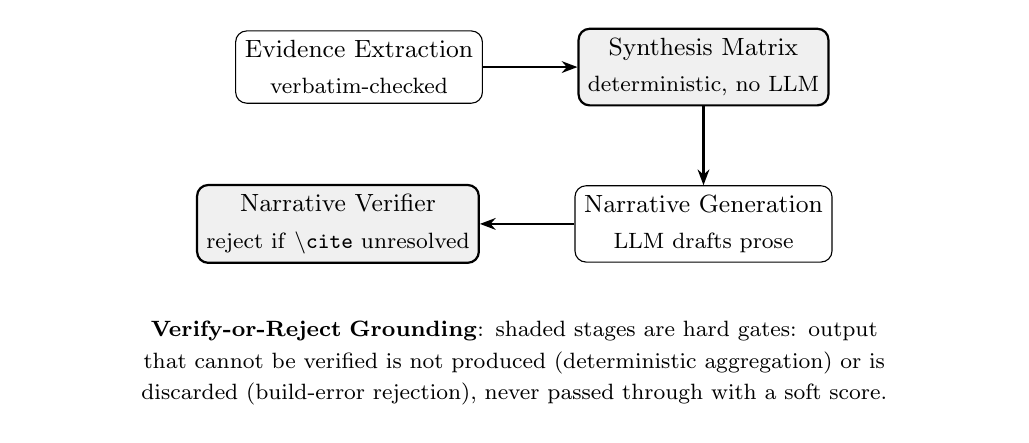
\begin{tikzpicture}[
 node distance=10mm and 12mm,
 box/.style={draw, rounded corners, minimum width=3.1cm, minimum height=9mm, align=center, font=\small},
 gate/.style={draw, rounded corners, minimum width=3.1cm, minimum height=9mm, align=center, font=\small, fill=gray!12, thick},
 arr/.style={-{Stealth[length=2mm]}, thick}
]
\node[box] (evi) {Evidence Extraction \\ \footnotesize verbatim-checked};
\node[gate, right=of evi] (mat) {Synthesis Matrix \\ \footnotesize deterministic, no LLM};
\node[box, below=of mat] (nar) {Narrative Generation \\ \footnotesize LLM drafts prose};
\node[gate, left=of nar] (ver) {Narrative Verifier \\ \footnotesize reject if \texttt{\textbackslash cite} unresolved};

\draw[arr] (evi) to (mat);
\draw[arr] (mat) to (nar);
\draw[arr] (nar) to (ver);

\node[fit=(ver)(nar), inner sep=0pt] (bottomrow) {};
\node[below=6mm of bottomrow, font=\footnotesize, align=center, text width=\linewidth]
 {\textbf{Verify-or-Reject Grounding}: shaded stages are hard gates: output that cannot be verified is not produced (deterministic aggregation) or is discarded (build-error rejection), never passed through with a soft score.};
\end{tikzpicture}
\caption{The evidence-grounded synthesis sub-pipeline. Shaded boxes are verify-or-reject gates; unshaded boxes are ordinary LLM-driven generation stages that feed into a gate.}
\label{fig:architecture}
\end{figure}

\section{Proposed Method: Verify-or-Reject Grounding}
\label{sec:method}

We define a pipeline stage as \textbf{scored-grounded} if it emits output alongside a confidence signal (a score, flag, or review-queue entry) that a downstream consumer may act on or ignore, and as \textbf{verify-or-reject grounded} if the stage's output type itself excludes unverifiable content: either because the stage is deterministic over already-verified inputs (introducing no new hallucination surface), or because an explicit verification step discards non-conforming output before it can propagate. The distinction matters because scored grounding is a property of the \emph{output}, inspectable but skippable, whereas verify-or-reject grounding is a property of the \emph{pipeline itself}, which a downstream stage cannot bypass by ignoring a score field it was never given -- the same reject-by-default logic behind the fail-safe-defaults principle in classical protection-system design~\cite{saltzer1975protection}, applied here to citation grounding instead of access control.

Algorithm~\ref{alg:vorg} formalizes the narrative-verification instance of the pattern used in \S\ref{sec:architecture}. Rather than checking each sentence against the evidence table by linear scan, as a naive scored-grounding implementation would, \textsc{VoRG-Certify} first compiles the evidence table into a hash index, then certifies the entire narrative in a single pass, so that certification cost scales with the size of the narrative and evidence table separately rather than with their product.

\captionof{algorithm}{\textsc{VoRG-Certify}: Linear-Time Verify-or-Reject Narrative Certification}
\label{alg:vorg}
\begin{algorithmic}[1]
\Require Evidence table $E = \{e_1, \dots, e_n\}$, each row keyed by a unique citation key $\kappa(e_i)$; generated narrative $N = (s_1, \dots, s_m)$
\Ensure Certified narrative $N'$ containing only sentences whose citations resolve to $E$; rejection log $R$ recording every discarded sentence and its cause
\Function{BuildIndex}{$E$}
 \State $H \gets$ empty hash map
 \For{each $e_i \in E$}
 \State $H[\kappa(e_i)] \gets e_i$ \Comment{expected $O(1)$ insert}
 \EndFor
 \State \Return $H$
\EndFunction
\Statex
\Function{Certify}{$N$, $H$}
 \State $N' \gets \emptyset$;\ $R \gets \emptyset$
 \For{each sentence $s_j \in N$} \Comment{single pass, $j = 1, \dots, m$}
 \State $K_j \gets \Call{ExtractKeys}{s_j}$ \Comment{one regex scan, $O(|s_j|)$}
 \If{$K_j = \emptyset$}
 \State $R \gets R \cup \{(s_j, \textsc{NoClaim})\}$ \Comment{no grounding claim at all}
 \ElsIf{$\exists\, k \in K_j$ such that $k \notin H$}
 \State $R \gets R \cup \{(s_j, \textsc{Unresolved})\}$ \Comment{build error, $O(1)$ lookup per key}
 \Else
 \State $N' \gets N' \cup \{s_j\}$
 \EndIf
 \EndFor
 \State \Return $(N', R)$
\EndFunction
\end{algorithmic}

\paragraph{Complexity.} Let $n = |E|$, let $m$ be the number of generated sentences, and let $M = \sum_{j=1}^m |s_j|$ be the total length of the narrative. \Call{BuildIndex}{} performs $n$ hash insertions, $O(n)$ expected time and $O(n)$ space for the index. \Call{Certify}{} makes one linear pass over $N$: key extraction is a single regex scan per sentence, contributing $O(M)$ in total across all sentences, and each extracted key is resolved against $H$ in expected $O(1)$, contributing $O(m)$ for the lookups. The full algorithm therefore runs in
\[
T(n, M) = O(n + M) \qquad \text{expected time,} \qquad S(n, m) = O(n + m) \qquad \text{auxiliary space,}
\]
since $m \le M$ and the output $N'$ and log $R$ together hold at most $m$ sentence references. This is linear in the combined size of the evidence table and the narrative and has no dependence on $n \cdot m$. The linear-scan alternative -- checking every sentence's citation against every evidence row, the implicit cost of a scored-grounding pipeline with no index structure -- costs $O(n \cdot m)$; \textsc{VoRG-Certify}'s hash-indexed design removes this quadratic term, which matters because $n$ and $m$ both grow with corpus size, so certification remains linear rather than quadratic as the evidence base scales. The same index-then-certify structure applies to contradiction judgments (indexed by claim-pair key, discarded below the Likert threshold rather than reported with a low score) and journal-metadata fields (indexed by source, tagged \texttt{unknown} when absent rather than interpolated), so the $O(n+M)$ bound extends to those subsystems under the same argument. Table~\ref{tab:contrast} contrasts the approach with the scored-grounding baseline typified by Li et al.~\cite{li2025enhancing}.

\begin{table}[h]
\centering
\caption{Scored grounding vs. verify-or-reject grounding.}
\label{tab:contrast}
\begin{tabular}{@{}p{3.6cm}p{5.3cm}p{5.3cm}@{}}
\toprule
& \textbf{Scored grounding} & \textbf{Verify-or-reject grounding} \\
\midrule
Unverifiable output & Emitted with a low score/flag & Not emitted; build error raised \\
Downstream dependence & Consumer must check the score & Consumer receives only verified output \\
Aggregation steps & Often LLM-driven, itself a hallucination source & Deterministic where possible (no new LLM surface) \\
Failure visibility & Silent unless score is inspected & Explicit, logged rejection \\
\bottomrule
\end{tabular}
\end{table}

\section{Evaluation}
\label{sec:evaluation}

\subsection{Research questions}

\begin{itemize}
 \item[\textbf{RQ1}] Does replacing each verify-or-reject gate with a matched
 confidence score, holding the stage decomposition fixed, change the rate at
 which unsupported or contradicted output reaches the final synthesis?
 \item[\textbf{RQ2}] Does the stage \emph{not} protected by a gate
 (research-gap detection) fail in a way the gated stages do not, and does the
 location of that failure line up with the architectural coverage described in
 \S\ref{sec:architecture}?
 \item[\textbf{RQ3}] How much of any measured claim-extraction gain is
 attributable to stage decomposition rather than to the LLM calls or the
 rejection mechanism?
\end{itemize}

\subsection{Setup}

Each topic is snapshotted once with the system's evaluation harness, freezing a
corpus so that no paper-source API traffic occurs during scored runs. Records
lacking a CrossRef abstract are backfilled from Semantic Scholar and OpenAlex
before freezing, and per-corpus abstract coverage is reported. Gold annotations
are authored by the present authors by independently correcting
pipeline-extracted claims against source abstracts and by independently judging
research-gap and contradiction labels against the corpus's own composition,
rather than by rubber-stamping the pipeline's output. We compare four
configurations, each repeated \NumRuns{} times (temperature 0.3, provider Groq
\texttt{openai/gpt-oss-120b} where an LLM call is used):

\begin{itemize}
 \item \textbf{Full pipeline (verify-or-reject).} All LLM-backed stages active;
 all three gates enforced.
 \item \textbf{Matched scored-grounding ablation.} Identical stage
 decomposition and LLM calls, but each of the three gates is replaced by a
 confidence score: unverifiable evidence fields are kept with a grounding
 score, unresolved narrative sentences are kept with a \texttt{citation\_resolved}
 flag, and below-threshold contradiction judgments are kept with their Likert
 score. This isolates rejection versus scoring on otherwise identical output
 (RQ1).
 \item \textbf{Pattern-mode ablation.} LLM-backed extraction stages replaced by
 regex/rule-based fallbacks, isolating dependence on the LLM calls (RQ3).
 \item \textbf{Naive baseline.} A single prompt containing all corpus
 abstracts/titles, asked in one shot for claims, contradictions, and gaps,
 scored with the identical matcher (RQ3).
\end{itemize}

Downstream-error metrics reported for every configuration:
\emph{unsupported sentences in the final narrative} (sentences with an
unresolved citation that nonetheless appear in the output; zero by construction
under verify-or-reject), \emph{retained false-positive contradictions} (asserted
contradictions matching a gold-negative pair), and \emph{unflagged metric
conflicts} (metric cells where sources disagree by more than 10\% with no
discrepancy flag).

\subsection{Pilot result (Topic 1)}
\label{sec:pilot}

The pilot topic is \textit{graph neural networks in drug discovery}; the frozen
corpus contains 10 papers retrieved from CrossRef. In the pilot snapshot only
one of the ten carried a non-empty abstract, limiting the independently
verifiable claim gold set to three sentences from a single paper; the
abstract-backfill step in the setup above was added in response to this and is
applied to all subsequent topics.

\begin{table}[h]
\centering
\caption{Claim-extraction performance on the pilot topic, mean $\pm$ SD over 3 runs, against 3 gold-annotated claims. Numbers are retained from the initial single-topic study and are underpowered at this gold-set size; see \S\ref{sec:threats}.}
\label{tab:claims}
\begin{tabular}{@{}lccc@{}}
\toprule
Configuration & Precision & Recall & F1 \\
\midrule
Full pipeline (verify-or-reject) & 0.294 $\pm$ 0.042 & 0.889 $\pm$ 0.192 & 0.442 $\pm$ 0.070 \\
Pattern-mode ablation & 0.439 $\pm$ 0.211 & 0.667 $\pm$ 0.000 & 0.510 $\pm$ 0.152 \\
Naive single-LLM baseline & 0.104 $\pm$ 0.006 & 0.333 $\pm$ 0.000 & 0.158 $\pm$ 0.007 \\
\bottomrule
\end{tabular}
\end{table}

On the pilot topic, both the full pipeline and the pattern-mode ablation
outperform the naive single-prompt baseline (F1 $2.8\times$ and $3.2\times$
higher), indicating that decomposing extraction into per-paper, per-claim stages
helps regardless of whether an LLM or a rule-based extractor performs each
stage. The pattern-mode point estimate is nominally higher than the full LLM
pipeline; with three near-verbatim gold sentences this favours a regex extractor
tuned to sentence boundaries, and the pattern-mode precision variance
($\pm 0.211$) is five times the full-pipeline variance ($\pm 0.042$),
consistent with a rule-based extractor whose hit rate depends on incidental
sentence structure. We therefore do not read the pilot F1 ordering as evidence
about rule-based versus LLM extraction in general (RQ3), and the multi-topic
study below is designed to settle it.

\textbf{Contradiction detection (pilot).} Across all nine pilot runs the
false-positive rate on the two hand-labelled negative pairs was 0.0. No
gold-positive contradictions exist in this small corpus, so recall is undefined;
this is a precision-only sanity check.

\textbf{Research-gap detection (pilot).} Gap recall against two independently
authored gold gaps was 0.0 in two of three full-pipeline runs and 0.5 in the
third (mean 0.17); precision@3 was 0.0 in every run. Inspecting the raw
predictions surfaces a concrete failure: one run's top-ranked gap claimed
\emph{``no studies have applied graph-based generative models \ldots for de novo
molecular generation''}, directly contradicted by the corpus's own sixth paper,
\emph{``Molecular generative Graph Neural Networks for Drug Discovery''}. The
gap-detection stage is the one component in \S\ref{sec:architecture} that does
\emph{not} apply verify-or-reject grounding: a candidate gap is generated and
ranked, but never checked against the titles or content of the corpus it is
judging.

\subsection{Multi-topic results}
\label{sec:multitopic}

% [PENDING] Fill from eval/results/matrix_<ts>/aggregate.md after running
%   python -m eval.run_matrix --topics <5 slugs> --modes llm,scored,pattern,baseline --repeats 5
% Insert here:
%   Table: pooled claim P/R/F1 per configuration across all topics (mean +/- SD).
%   Table: per-topic F1 to show whether the pilot pattern-vs-LLM ordering holds.
%   Prose: state whether decomposition gain (RQ3) replicates and whether the
%          pattern-mode advantage was a small-gold-set artefact.

\subsection{Scored-grounding ablation (RQ1)}
\label{sec:scoredablation}

% [PENDING] Fill from the same aggregate.md (scored vs llm columns). Insert:
%   Table: unsupported_sentences_in_narrative, retained_fp_contradictions,
%          unflagged_metric_conflicts -- verify-or-reject (=0 by construction)
%          vs matched scored-grounding, pooled across topics, mean +/- SD.
%   Prose: quantify how many unsupported statements reach the final synthesis
%          once the gate is replaced by a score, and relate to RQ1.

\subsection{Gap-to-failure correspondence (RQ2)}
\label{sec:gaptofailure}

% [PENDING] Aggregate the gap-detection failures across all topics. Report, per
% topic: number of confirmed false-positive gaps (contradicted by a corpus
% paper) from the ungated gap stage, vs confirmed false output from the two
% gated stages (expected 0). This is the paper's central claim -- state it as a
% correspondence between architectural coverage and failure location, with n =
% (topics x runs) now large enough to not rest on a single incident.

\subsection{Cost}

Mean cost per full-pipeline run on the pilot topic was \$0.008 $\pm$ \$0.002
(16.3 $\pm$ 1.5 LLM calls), against \$0.002 $\pm$ \$0.001 for the pattern-mode
ablation and \$0.001 (1 call) for the naive baseline. The matched
scored-grounding ablation issues the same LLM calls as the full pipeline and
therefore costs the same to within noise; the difference is in what its output
type permits, not in compute. % [PENDING] replace with pooled multi-topic cost.

\section{Discussion}
\label{sec:discussion}

The gated and ungated stages diverge in the way the architecture predicts.
Claim extraction and contradiction detection each pass every candidate output
through an explicit accept/reject check before it can be reported, and neither
produced output contradicted by the reviewed corpus. Research-gap detection has
no equivalent check -- a candidate gap is generated and ranked but never
compared against the corpus it is judging -- and it is precisely there that the
pipeline produced a false claim contradicted by a paper already in that corpus.
This correspondence was not constructed as a test of VoRG; it emerged during
evaluation of the existing pipeline, and the location of the failure lines up
with the one architectural gap identified in \S\ref{sec:architecture}. We treat
this correspondence, rather than the claim-extraction F1 numbers, as the
strongest evidence in the paper for build-time rejection over post-hoc scoring.

The journal-metadata reconciliation component illustrates the same discipline
applied to structured rather than narrative output: values are classified as
verified, estimated, or unknown, and differences between sources are surfaced in
a discrepancy field rather than silently averaged. Nothing about the underlying
idea is specific to literature review -- any pipeline that generates text or
structured records from retrieved sources can apply the same accept/reject check
before passing output downstream, in place of a confidence score a later stage
might not act on.

The results do not show that verify-or-reject grounding solves hallucination in
every setting. What the evaluation establishes is where verification is already
load-bearing and where its absence produces a concrete, corpus-contradicted
failure. Extending the gate to research-gap detection, and testing the pattern
on larger and more varied corpora, are the most direct next steps.

\section{Threats to Validity}
\label{sec:threats}
\label{sec:limitations}

\textbf{Construct validity.} The matched scored-grounding ablation is our
operationalisation of ``the same pipeline without the gate''. It holds the
stage decomposition and the LLM calls fixed and varies only the accept/reject
versus score decision; a different scored-grounding implementation could behave
differently, and the naive single-prompt baseline tests only decomposition, not
scoring.

\textbf{Internal validity.} Two pre-existing implementation defects were
identified and fixed during evaluation, and the reported results reflect the
corrected implementation.\footnote{A retired LLM model identifier that caused
fallback to a degraded extraction mode, and a schema-validation issue that
rejected valid null-valued fields from certain LLM providers.} LLM providers
are non-deterministic even at low temperature; we report mean and SD over
\NumRuns{} runs per configuration and pin the provider, model, and temperature.

\textbf{Statistical conclusion validity.} The pilot claim-extraction gold set
(Table~\ref{tab:claims}) contains three sentences; its variance estimates are
indicative only and its F1 ordering is not used to draw conclusions about
extractor type. The multi-topic study (\S\ref{sec:multitopic}) is designed to
provide the statistical power the pilot lacks.

\textbf{External validity.} % [PENDING: state final topic count and domains]
The evaluation covers a small number of gold-annotated topics and a single
annotator team; results should be read as evidence that the architecture
behaves as predicted on these corpora, not as a guarantee that effect sizes
generalise across all of scientific NLP. Several supporting citations carry
explicit quartile caveats because Q1 status could not be independently confirmed
for every subtopic at the time of writing.

\section{Reproducibility}
\label{sec:repro}

The reference implementation, evaluation harness, frozen corpora, gold-annotation
files, and the \texttt{run\_matrix} driver used for \S\ref{sec:multitopic} are
released at the repository below. Each results directory records the repository
commit hash, the LLM provider and model, the temperature, per-topic abstract
coverage, per-run cost, and parse-failure counts. All scored runs use the frozen
corpus snapshots, so re-running the evaluation issues no traffic to paper
sources and depends only on the pinned LLM endpoint.

\section{Conclusion}

We described Verify-or-Reject Grounding, an architectural pattern that treats
citation grounding as a build-time invariant rather than a scored property, gave
a linear-time certification algorithm for its narrative-verification instance,
and implemented it across evidence-grounded synthesis, contradiction detection,
and journal-metadata reconciliation in an eight-stage research-assistant
pipeline.

The evaluation's most robust result is a correspondence between architectural
coverage and failure location: the stages protected by a verify-or-reject gate
produced no output contradicted by the reviewed corpus, while research-gap
detection, the one major unprotected stage, produced a confirmed false claim
that a corpus paper directly contradicts. A matched scored-grounding ablation,
holding the stage decomposition fixed and replacing each rejection with a
confidence score, % [PENDING: one-sentence headline result from \S\ref{sec:scoredablation}]
quantifies how much unsupported output reaches the final synthesis once the gate
is removed.

Future work will (i) apply the verify-or-reject mechanism to research-gap
detection, closing the one architectural gap identified here; (ii) broaden the
evaluation corpus and annotator pool; and (iii) test whether the gap-to-failure
correspondence holds across scientific domains beyond the topics studied here.

\section*{Data and Code Availability}

The reference implementation, evaluation harness, and gold-annotation files are
available at \url{https://github.com/harishvidyarthcsecs/Research}.

\section*{Conflict of Interest}

The authors declare no conflict of interest.

\bibliographystyle{unsrt}
\bibliography{references}

\end{document}
